\subsection{Data Sources, Modeling choices}

We use the AME model on the two aforementioned measures of state amity to generate a combined measure of state preference similarity which accounts for network effects. We use the distance between states' ideal points (as calculated by \citet{voeten:XXXX} using UN data) and S-score for two states alliance portfolios. However, to facilitate comparison between the metrics, we first transform the S-score into a measure of distance between alliance portfolios.\footnote{D = 1 - S} We then standardize and normalize these two measures. This gives us an N by N by Y by 2 array, where the first two dimensions represent countries, the third dimension is the year, and the fourth is the particular measure of similarity. So the item at index (1,2,1,1) would be the transformed value of the S-score for countries XXX and YYY at the first year of our data (YYYY), similarly (1,2,1,2) would be the UN ideal point distance.

Another important question is the amount of temporal aggregation used. In our baseline model, we treat each year as separate and gain a unique observation of each states ideal point in each year. However, this raises a real risk of temporal inconsistency in the values. An alternative approach would be to have a rolling average for the measures of similarity over a number of years. This would allow us to infer a country's relative position not just by their behavior in a given year, but also their behavior in the past few years. The risk if we use too much temporal aggregation is that we are including data which is no longer relevant to a country's relative preferences. For instance, Turkey and Russia's relationship looks a lot more positive when we look at 2013 and 2014 then when we look at 2015. To that end, in addition to our baseline model where years are seen as independent, we also evaluate models where ... 

With this data, we run an AME model with a Gaussian link, and in particular we use the uDv term to estimate each states position in a two-dimensional latent space. We then evaluate whether their is additional utility gained from using this latent position, as compared to the component measures of similarity of alliance portfolio and UN ideal point distance.

\section{Constructing Latent Angle Measure}

\begin{figure}[ht]
	\centering
	\includegraphics[width=.7\textwidth]{latPlot}
	\caption{Latent factor plot.}
	\label{fig:latPlot}
\end{figure}

\subsection{Face Plausibility}

Are states close to who we'd expect them to be?

\subsection{Temporal Reliability}

Are our measures consistent?

\section{Model Competition}

\subsection{Data, Controls}

\subsection{In sample explanation}

Are coeffs starry and in right direction

\begin{figure}[ht]
	\centering
	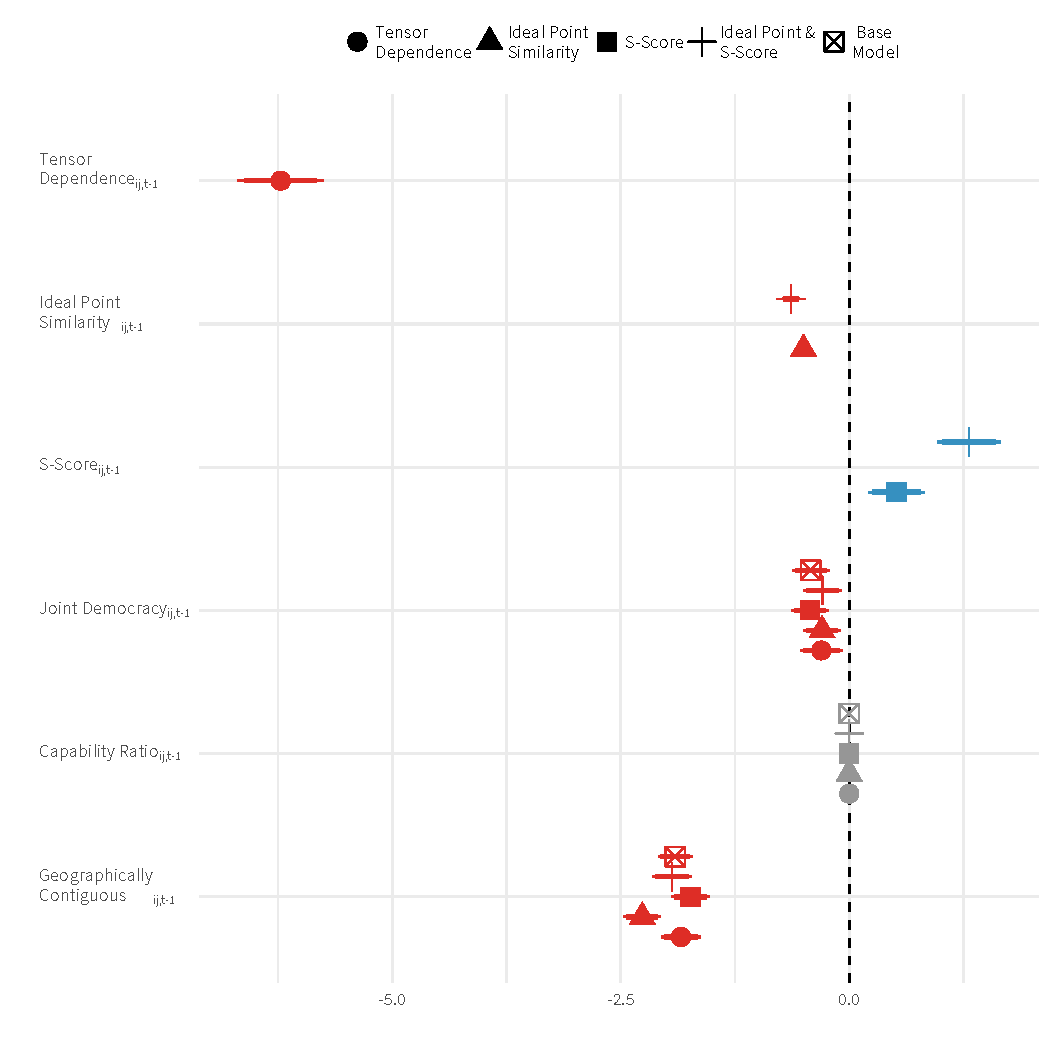
\includegraphics[width=.7\textwidth]{betaEst}
	\caption{Parameter estimates from models with different measures of state preference. Point represents average estimate, line through the point represents the 95\% confidence interval.}
	\label{fig:coefP}
\end{figure}
\FloatBarrier

\subsection{Out of sample prediction}

\begin{figure}[ht]
	\centering
	\begin{tabular}{cc}
	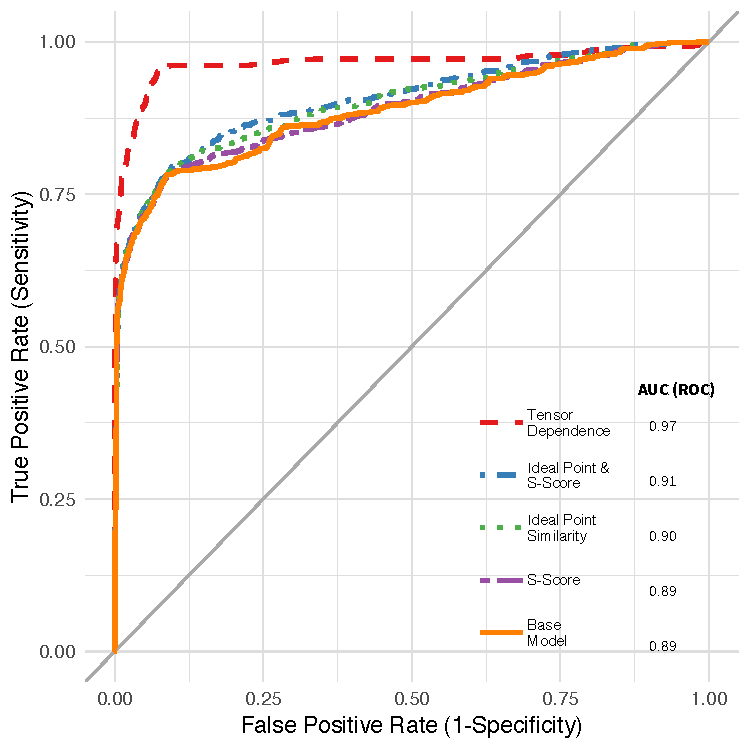
\includegraphics[width=.5\textwidth]{roc_outSample} & 
	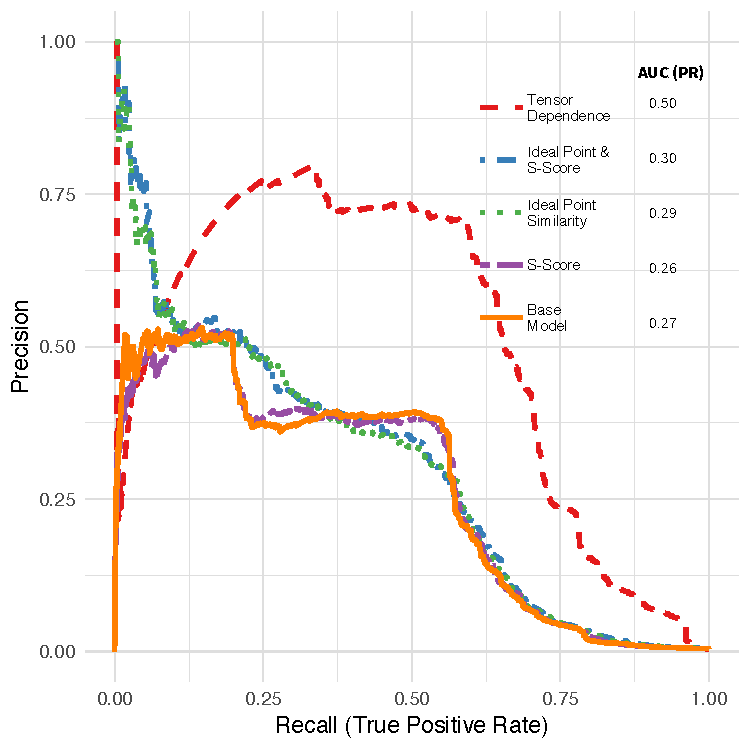
\includegraphics[width=.5\textwidth]{rocPr_outSample}	
	\end{tabular}
	\caption{Assessments of out-of-sample predictive performance using ROC curves and PR curves. AUC statistics are provided as well for both curves.}
	\label{fig:roc}
\end{figure}
\FloatBarrier

Are we right? Yes.
